\documentclass[10pt]{beamer}
\usetheme{metropolis}

\usepackage{amsmath,amssymb}
\usepackage{mathtools}
\usepackage{xeCJK}
\setCJKmainfont{Noto Serif SC}
\usepackage{tikz-cd}
\usepackage{graphicx}

% 1. 开启标题背景色填充
\metroset{block=fill}

% theorem environments
\newtheorem{proposition}{Proposition}
\newtheorem{exercise}{Exercise}

% notation
\newcommand{\R}{\mathbb{R}}
\newcommand{\N}{\mathbb{N}}
\newcommand{\F}{\mathcal{F}}
\newcommand{\supp}{\operatorname{supp}}

\title{Ch8\quad Submanifolds, Diffeomorphisms, and the Inverse Function Theorem}
\subtitle{Immersions, Submersions, Embeddings \& Regular Submanifolds}
\date{October 22, 2026}
\author{LXJ}

\begin{document}

\maketitle

%====================================================================
\section{Immersions, Submersions and Embeddings}

\begin{frame}{Maps between manifolds}
	Let $\Psi : M \to N$ be a $C^\infty$ map. Recall that the
	differential $\Psi_{*,m} : T_m M \to T_{\Psi(m)} N$ is a linear map.
	\begin{definition}
		$\Psi$ is called
		\begin{enumerate}
			\item an \alert{immersion} \textbf{(浸入)} if $\Psi_{*,m}$
			      is non-singular for all $m \in M$, i.e.\
			      $\ker \Psi_{*,m} = \{0\} \subset T_m M$;
			\item a \alert{submersion} \textbf{(淹没)} if $\Psi_{*,m}$
			      is a surjective map for all $m \in M$;
			\item an \alert{embedding} \textbf{(嵌入)} if $\Psi$ is an
			      immersion and also one-to-one, and
			      $\Psi : M \to \Psi(M) \subset N$ is a homeomorphism
			      with $\Psi(M)$ carrying the relative topology;
			\item a \alert{diffeomorphism} if $\Psi$ is one-to-one,
			      onto, and $\Psi^{-1}$ is also $C^\infty$.
		\end{enumerate}
	\end{definition}
\end{frame}

\begin{frame}{Submanifolds}
	\begin{definition}
		Let $M$, $N$ be $C^\infty$-manifolds.
		\begin{enumerate}
			\item If $M$ is a subset of $N$，and
			      the inclusion map $\iota: M\to N$ is an immersion, then $M$ is called
			      an \emph{immersed  submanifold} of $N$.
			\item If the inclusion map
			      $\iota: M\to N$ is an embedding, then $M$ is called a \emph{regular
				      submanifold} of $N$.
		\end{enumerate}
	\end{definition}
\end{frame}

\begin{frame}{Submanifolds}
	\begin{lemma}
		Let $M$ and $N$ be $C^\infty$-map. Let $f:M\to N$ be a $C^\infty$-map.
		\begin{enumerate}
			\item If $f$ is an injective immersion, considering $f(M)$ as a manifold
			      with the topology inherited from $M$, then $f(M)$ is an immersed submanifold of $N$;
			\item If $f$ is an embedding ($f(M)$ has a topology inherited from $N$), then $f(M)$ is
			      a regular manifold of $N$.
		\end{enumerate}
	\end{lemma}
\end{frame}


\begin{frame}{Immersions of the real line into the plane}
	\begin{center}
		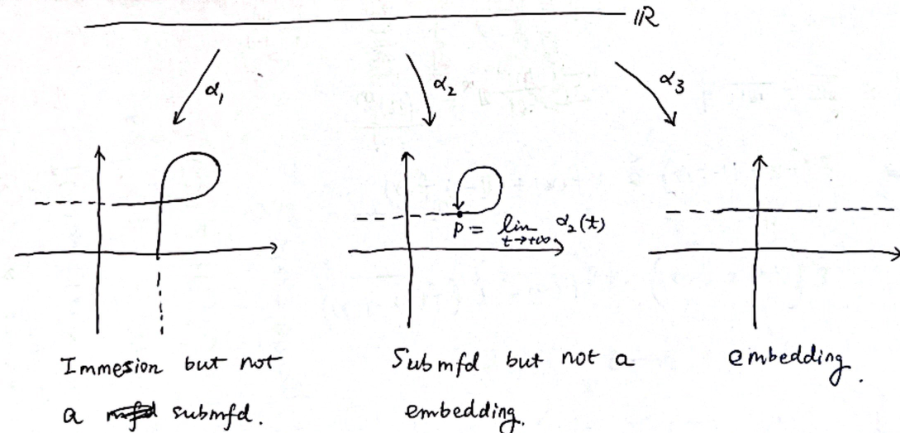
\includegraphics[width=0.85\textwidth]{fig_immersion.png}
	\end{center}
	\begin{itemize}
		\item $\alpha_1$: immersion but not a regular submanifold;
		\item $\alpha_2$: image is a submanifold but $\alpha_2$ is
		      not an embedding ($p = \lim_{t \to +\infty} \alpha_2(t)$);
		\item $\alpha_3$: embedding.
	\end{itemize}
\end{frame}

\begin{frame}{Remarks on diffeomorphisms}
	\begin{block}{Remark}
		Suppose $M$ and $N$ are diffeomorphic. Then $N$ and $M$
		are diffeomorphic. It is clear that being diffeomorphic is
		an equivalence relation.
	\end{block}
	\medskip
	\begin{itemize}
		\item \textbf{Milnor} proved that $S^7$ has a differentiable
		      structure which is \emph{not} diffeomorphic to the usual
		      one (exotic spheres).
		\item There are also locally Euclidean spaces with \emph{no}
		      differentiable structures at all.
	\end{itemize}
\end{frame}

%====================================================================
\section{Examples}

\begin{frame}{Examples (1--3)}
	\begin{exampleblock}{Eg 1}
		The inclusion $\iota : S^1 \longrightarrow \R^2$ is an
		embedding.
	\end{exampleblock}
	\begin{exampleblock}{Eg 2}
		$f : \R \to \R^2$, $t \longmapsto (\cos t, \sin t)$ is an
		immersion but not an embedding (not one-to-one).
	\end{exampleblock}
	\begin{exampleblock}{Eg 3 (Injective immersion)}
		$f : \R \to \R^2$,
		\[
			t \longmapsto
			\left( \frac{t^3 + t}{t^4 + 1},\ \frac{t^3 - t}{t^4 + 1}
			\right) \qquad (t \in \R).
		\]
		$f$ is one-to-one and $f_*$ is non-singular, but $f$ is not a
		homeomorphism between $\R$ and $f(\R)$ because $f(\R)$ is
		compact. Hence $f$ is not an embedding.
	\end{exampleblock}
\end{frame}

\begin{frame}{Examples (4--6)}
	\begin{exampleblock}{Eg 4 (Embedding of the torus)}
		$f : T^2 = S^1 \times S^1 \to \R^3$,
		\[
			(e^{i\theta}, e^{i\varphi}) \longmapsto
			\bigl( (a + b\cos\varphi)\cos\theta,\,
			(a + b\cos\varphi)\sin\theta,\, b\sin\varphi \bigr).
		\]
		$f$ is a smooth embedding; $f(T^2)$ is a torus in $\R^3$.
	\end{exampleblock}
	\begin{exampleblock}{Eg 5 (Standard embedding, $m \le n$)}
		$f : \R^m \to \R^n$,\quad
		$(x^1, \dots, x^m) \longmapsto (x^1, \dots, x^m, 0, \dots, 0)$.
	\end{exampleblock}
	\begin{exampleblock}{Eg 6 (Standard submersion, $m > n$)}
		$f : \R^m \to \R^n$,\quad
		$(x^1, \dots, x^m) \longmapsto (x^1, \dots, x^n)$.
	\end{exampleblock}
\end{frame}

%====================================================================
\section{Normal Form for an Immersion}

\begin{frame}{The local normal form for an immersion}
	\begin{theorem}
		Let $f : M^m \to N^n$ be an immersion, i.e.\
		$\ker f_{*p} = \{0\}$ for all $p \in M$ ($m \le n$). For any
		$p \in M$, $f(p) = q \in N$, there exist local coordinate
		systems $(U, \varphi)$ about $p$ and $(V, \psi)$ about $q$
		s.t.
		\[
			\psi \circ f \circ \varphi^{-1}(x_1, \dots, x_m)
			= (x_1, \dots, x_m, 0, \dots, 0).
		\]
	\end{theorem}
	\medskip
	Locally, an immersion looks like the \emph{standard embedding} of
	$\R^m$ into $\R^n$.
\end{frame}

\begin{frame}{Proof of the normal form for an immersion (I)}
	Given arbitrary local coordinate systems $(\widetilde{U},
		\widetilde{\varphi})$ and $(\widetilde{V}, \widetilde{\psi})$
	about $p$ and $q$, the local form for $f_*$ is given by
	\[
		f_*\left( \frac{\partial}{\partial x_i} \right)
		= \sum_{j=1}^{n}
		\left. \frac{\partial (y_j \circ f \circ
			\widetilde{\varphi}^{-1})}{\partial x_i} \right|_{\varphi(p)}
		\left. \frac{\partial}{\partial y_j} \right|_{f(p)} .
	\]
	So the Jacobian of $f_*$ is $D\widetilde{\psi} \circ f_*
		\widetilde{\varphi}^{-1}\big|_{\widetilde{\varphi}(p)}$. Write
	$F \triangleq \widetilde{\psi} \circ f \circ
		\widetilde{\varphi}^{-1}$. WLOG we can assume
	\[
		\left( \frac{\partial F_i}{\partial x_j}
		\right)_{1 \le i \le m,\ 1 \le j \le m}
		\quad \text{is non-degenerate.}
	\]
\end{frame}

\begin{frame}{Proof of the normal form for an immersion (II)}
	Define the map
	\[
		\Phi(x_1, \dots, x_m, x_{m+1}, \dots, x_n)
		\triangleq
		\begin{pmatrix}
			F_1(x_1, \dots, x_m)               \\
			\vdots                             \\
			F_m(x_1, \dots, x_m)               \\
			F_{m+1}(x_1, \dots, x_m) + x_{m+1} \\
			\vdots                             \\
			F_n(x_1, \dots, x_m) + x_n
		\end{pmatrix}.
	\]
	Then
	\[
		D\Phi =
		\begin{pmatrix}
			\left( \dfrac{\partial F_i}{\partial x_j} \right)_{m \times m} & 0       \\
			*                                                              & I_{n-m}
		\end{pmatrix}
	\]
	is non-degenerate.
\end{frame}

\begin{frame}{Proof of the normal form for an immersion (III)}
	Therefore there are open subsets
	$U \subset \widetilde{\varphi}(\widetilde{U})$,
	$V \subset \widetilde{\psi}(\widetilde{V})$ such that
	$\Phi\big|_U : U \to V$ is a diffeomorphism, and
	\[
		(x_1, \dots, x_m, 0, \dots, 0)
		\xleftrightarrow{\ \text{one-to-one}\ }
		\begin{pmatrix} F_1 \\ \vdots \\ F_n \end{pmatrix}.
	\]
	If we consider the composition $\Phi^{-1} \circ F$, then it is
	clear that
	\[
		\Phi^{-1} \circ F(x_1, \dots, x_m)
		= (x_1, x_2, \dots, x_m, 0, \dots, 0). \qedhere
	\]
\end{frame}

%====================================================================
\section{Normal Form for a Submersion}

\begin{frame}{The local normal form for a submersion}
	\begin{theorem}
		Let $f : M^m \to N^n$ be a submersion, i.e.\ $f_{*p}$ is
		surjective ($m \ge n$). Then for all $p \in M$ and
		$q = f(p) \in N$, there are local coordinate systems
		$(U, \varphi)$ and $(V, \psi)$ s.t.\ $\psi \circ f \circ
			\varphi^{-1} : \varphi(U) \to \psi(V)$ is given by
		\[
			\psi \circ f \circ \varphi^{-1}(x_1, \dots, x_m)
			= (x_1, \dots, x_n).
		\]
	\end{theorem}
	\medskip
	Locally, a submersion looks like the \emph{standard submersion} of
	$\R^m$ onto $\R^n$.
\end{frame}

\begin{frame}{Proof of the normal form for a submersion (I)}
	For all $p \in M$ and $q = f(p) \in N$, take arbitrary local
	coordinate systems $(\widetilde{U}, \widetilde{\varphi})$ of $p$
	and $(\widetilde{V}, \widetilde{\psi})$ of $q$. Define
	\[
		F = \widetilde{\psi} \circ f \circ \widetilde{\varphi}^{-1}
		: \widetilde{\varphi}(\widetilde{U})
		\longrightarrow \widetilde{\psi}(\widetilde{V}).
	\]
	Since $f_*$ is a surjective map,
	$DF = \left( \dfrac{\partial F_i}{\partial x_j}
		\right)_{1 \le i \le n,\ 1 \le j \le m}$ has full rank ($n$).
	\medskip

	Assume $\left( \dfrac{\partial F_i}{\partial x_j}
		\right)_{1 \le i \le n,\ 1 \le j \le n}$ is non-degenerate.
	Then define the map
	\[
		\Phi(x_1; \dots; x_m) =
		\begin{pmatrix}
			F_1 \\ \vdots \\ F_n \\ x_{n+1} \\ \vdots \\ x_m
		\end{pmatrix}
		=
		\begin{pmatrix}\widetilde{y}_1 \\ \vdots \\ \widetilde{y}_m
		\end{pmatrix}.
	\]
\end{frame}

\begin{frame}{Proof of the normal form for a submersion (II)}
	Then
	\[
		D\Phi =
		\begin{pmatrix}
			\left( \dfrac{\partial F_i}{\partial x_j} \right)_{n \times n} & *       \\
			0                                                              & I_{m-n}
		\end{pmatrix}
	\]
	is non-degenerate. Therefore
	\[
		\Phi^{-1}(\widetilde{y}_1, \dots, \widetilde{y}_m)
		= (x_1, \dots, x_m), \qquad
		\Phi \circ \Phi^{-1}(\widetilde{y}_1, \dots, \widetilde{y}_m)
		= (\widetilde{y}_1, \dots, \widetilde{y}_m),
	\]
	\[
		\Longrightarrow\quad
		F \circ \Phi^{-1}(\widetilde{y}_1, \dots, \widetilde{y}_m)
		= (\widetilde{y}_1, \dots, \widetilde{y}_n)
		= \bigl( F_1(x_1, \dots, x_m), \dots, F_n(x_1, \dots, x_m)
		\bigr).
	\]
	So
	\[
		\psi \circ f \circ \widetilde{\varphi}^{-1} \circ
		\Phi^{-1}(\widetilde{y}_1, \dots, \widetilde{y}_n)
		= (\widetilde{y}_1, \dots, \widetilde{y}_n). \qedhere
	\]
\end{frame}

%====================================================================
\section{Structure Theorem for Regular Submanifolds}

\begin{frame}{The structure theorem}
	\begin{center}
		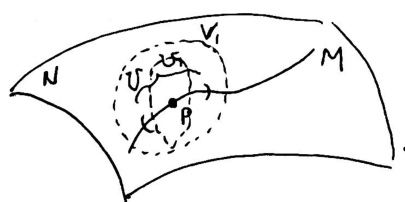
\includegraphics[height=0.28\textheight]{fig_submfd_struct.png}
	\end{center}
	\begin{theorem}
		$M^m$ is a regular submanifold of $N^n$ $\iff$ $M$ is a
		subtopological space of $N$, and for all $p \in M$ there
		exists a local coordinate system $(U, \varphi)$ of $N$ with
		coordinate functions $(x_1, \dots, x_n)$ s.t.
		\[
			M \cap U = \{ b \in U \mid x_i(b) = 0
			\ \text{for } m+1 \le i \le n \}.
		\]
	\end{theorem}
	i.e.\ locally $M$ is cut out of $N$ by the vanishing of the
	last $n - m$ coordinate functions.
\end{frame}

\begin{frame}{Proof: embedding $\Rightarrow$ slice condition}
	Since $\iota : M \to N$ is an embedding, it is an immersion and a
	one-to-one map, and $M$ is diffeomorphic to $\iota(M)$ with the
	subspace topology. By the local normal form for immersions, there
	are local coordinate systems $(U_1, \varphi_1)$ of $p \in M$ and
	$(V_1, \psi_1)$ of $p \in N$ s.t.
	\[
		\psi_1 \circ \iota \circ \varphi_1^{-1}(x_1, \dots, x_m)
		= (x_1, \dots, x_m, 0, \dots, 0).
	\]
	Assume $\psi_1(q) = (x_1(q), \dots, x_n(q))$, $q \in V_1$. Let
	\[
		V_1' = \{ q \in V_1 \mid (x_1(q), \dots, x_m(q))
		\in \varphi_1(U_1) \} \subset V_1.
	\]
\end{frame}

\begin{frame}{Proof: shrinking the neighborhood}
	If we take the open set $U \subset V_1'$ of $N$ such that
	$M \cap U \subset U_1$, then $(V_1, \psi_1)$ restricts to
	$(U, \psi_1)$ as a local coordinate system on $N$. For
	$q \in M \cap U \ (\subset U_1)$:
	\[
		x_{m+1}(q) = \dots = x_n(q) = 0, \qquad
		(x_1(q), \dots, x_m(q)) \in \varphi_1(U_1).
	\]
	Let $q' = \varphi_1^{-1}\bigl( x_1(q), \dots, x_m(q) \bigr)
		\in U_1$. Then
	\begin{align*}
		\psi_1(q')
		 & = \psi_1 \circ \iota \circ \varphi_1^{-1}
		\bigl( x_1(q), \dots, x_m(q) \bigr)                          \\
		 & = \bigl( x_1(q), \dots, x_m(q), 0, \dots, 0 \bigr)        \\
		 & = \bigl( x_1(q), \dots, x_m(q), x_{m+1}(q), \dots, x_n(q)
		\bigr) = \psi_1(q).
	\end{align*}
	Since $\psi_1$ is one-to-one, $q = q' \in U_1 \subset M$. Hence
	$\{ b \in U \mid x_{m+1}(b) = \dots = x_n(b) = 0 \} \subset M
		\cap U$.
\end{frame}

\begin{frame}{Proof: slice condition $\Rightarrow$ embedding}
	If $M$ satisfies: for all $p \in M$ there exists
	$(U; x_1, \dots, x_n)$ of $p \in N$ s.t.
	\[
		M \cap U = \{ b \in U \mid x_{m+1}(b) = \dots = x_n(b) = 0 \},
	\]
	then $M$ is a local Euclidean space, with $M \cap U$ described by
	the coordinates $\{ x_1(b), \dots, x_m(b) \}$. Furthermore, $M$
	is a differentiable manifold, and the inclusion $\iota : M \to N$
	is given by
	\[
		(x_1, \dots, x_m) \longmapsto (x_1, \dots, x_m, 0, \dots, 0),
	\]
	which has full rank and is an embedding. \qedhere
\end{frame}

%====================================================================
\section{The Constant Rank Theorem}

\begin{frame}{The constant rank theorem}
	\begin{theorem}[Constant Rank]
		If $f : M^m \to N^n$ is a smooth map, and there exists a
		constant $l$ s.t.\ $\operatorname{rank} f_{*p} = l$ for all
		$p \in M$, then for all $q \in N$, $f^{-1}(\{q\})$ is either
		$\varnothing$ or a regular submanifold of $M$, with dimension
		$m - l$.
	\end{theorem}
	\begin{proof}
		Let $S = f^{-1}(\{q\}) \subset M$; assume $S \neq \varnothing$.
		For all $p \in S \subset M$, let $q = f(p) \in N$. Then there
		are local coordinate systems $(U, \varphi)$ and $(V, \psi)$
		s.t.\ $\varphi(p) = 0 \in \R^m$, $\psi(q) = 0 \in \R^n$, and
		\[
			\psi \circ f \circ \varphi^{-1}
			: \varphi(U) \longrightarrow \psi(V)
		\]
		\[
			(x_1, \dots, x_m) \longmapsto
			\bigl( x_1, \dots, x_l,\ g_{l+1}(x_1, \dots, x_l), \dots,
			g_n(x_1, \dots, x_l) \bigr).
		\]
	\end{proof}
\end{frame}

\begin{frame}{Proof of the constant rank theorem (I)}
	To prove this, consider $F : \R^m \to \R^n$ of rank $l$. Assume
	$\left( \dfrac{\partial F_i}{\partial x_j}
		\right)_{1 \le i, j \le l}$ is non-degenerate. Define
	\[
		\Phi(x_1, \dots, x_m) =
		\begin{pmatrix}
			F_1 \\ \vdots \\ F_l \\ x_{l+1} \\ \vdots \\ x_m
		\end{pmatrix}
		\ \Longrightarrow\
		D\Phi \ \text{is non-degenerate.}
	\]
	Since $\Phi \circ \Phi^{-1}(y_1, \dots, y_m) = (y_1, \dots, y_m)$,
	\[
		F \circ \Phi^{-1}(y_1, \dots, y_m)
		= F(x_1, \dots, x_m)
		= \begin{pmatrix}
			F_1(x_1, \dots, x_m) \\ \vdots \\ F_n(x_1, \dots, x_m)
		\end{pmatrix}
		\triangleq
		\begin{pmatrix}
			y_1 \\ \vdots \\ y_l \\ g_{l+1}(x_1, \dots, x_m) \\
			\vdots
		\end{pmatrix}.
	\]
\end{frame}

\begin{frame}{Proof of the constant rank theorem (II)}
	Because $\operatorname{rank} D(F \circ \Phi^{-1}) = l
		= \operatorname{rank} DF$,
	\[
		\frac{\partial g_i}{\partial y_j} = 0 \qquad
		\forall\, i = l+1, \dots, n,\ \forall\, j = l+1, \dots, m,
	\]
	so $g_{l+1}(y_1, \dots, y_l), \dots, g_n(y_1, \dots, y_l)$ depend
	only on $y_1, \dots, y_l$.
	\medskip

	Therefore there exists an open set $U \subset M$ s.t.
	\begin{align*}
		S \cap U
		 & = \{ s \in U \mid y_i(s) = 0 \text{ for } 0 < i \le l \} \\
		 & = \{ s \in U \mid y_1(s) = \dots = y_l(s) = 0, \
		g_{l+1}(y_1, \dots, y_l) = 0, \dots, g_n(y_1, \dots, y_l) = 0
		\}.
	\end{align*}
	By the structure theorem for regular submanifolds, $S$ is a
	regular submanifold of $M$ of dimension $m - l$. \qedhere
\end{frame}

\end{document}
